\documentclass[12pt,a4paper]{article}
\usepackage[a4paper, left=2.5cm,right=2.5cm,top=3cm,bottom=3cm]{geometry}
\usepackage[utf8]{inputenc}
\usepackage[spanish]{babel}
\addto\captionsspanish{
	\renewcommand\chaptername{}
	\renewcommand\appendixname{Anexo}
	\renewcommand\appendixpagename{Anexos}
	\def\tablename{Tabla}
	\def\listtablename{\'Indice de tablas}
}
\usepackage{ucs}
\usepackage{subfig}
\usepackage{float}
\usepackage{amsmath}
\usepackage{amsfonts}
\usepackage{amssymb}
\usepackage{graphicx}
\usepackage{listings}
\usepackage{color}
\usepackage[T1]{fontenc}
\usepackage[scaled]{beramono}
\usepackage{upquote}
\usepackage{xcolor}
\usepackage{listings}
\usepackage{caption}
\usepackage{chngcntr}
\usepackage{endnotes}
\usepackage{float}
\usepackage{hyperref}
\usepackage{wrapfig}
\usepackage{fancyhdr}
\usepackage{emptypage}
\usepackage{times}
\usepackage{array}
\usepackage{setspace}
\usepackage{multirow}
%\usepackage{subfigure}
\usepackage{verbatim}
%\usepackage{tabulary}
%\usepackage{graphicx,subfigure}
\usepackage[bottom]{footmisc} 
\usepackage{appendix}
\usepackage{mathtools}
\usepackage{textcomp}


%listing, code style
% Define a custom color
\definecolor{backcolour}{rgb}{0.95,0.95,0.92}
\definecolor{codegreen}{rgb}{0,0.6,0}

% Define listing style
\lstset{
	language=python,
	tabsize=4,
	rulecolor=,
	basicstyle=\scriptsize,
	upquote=true,
	aboveskip={1.2\baselineskip},
	columns=fixed,
	numbers=left,
	showstringspaces=false,
	extendedchars=true,
	breaklines=true,
	prebreak = \raisebox{0ex}[0ex][0ex]{\ensuremath{\hookleftarrow}},
	showtabs=false,
	showspaces=false,
	showstringspaces=false,
	identifierstyle=\ttfamily,
	keywordstyle=\color[rgb]{0,0,1},
	commentstyle=\color[rgb]{0.133,0.545,0.133},
	stringstyle=\color[rgb]{0.627,0.126,0.941},
} 


\renewcommand{\notesname}{Fuentes}
\renewcommand{\baselinestretch}{1.2}
\hypersetup{
	colorlinks,%
	citecolor=black,%
	filecolor=black,%
	linkcolor=black,%
	urlcolor=black
}

\begin{document}
	
\begin{titlepage}
	\centering
	%\null\vfill
	
\includegraphics[width=\textwidth]{FIGURES/Portada/Logo_portada.png} 
	\vspace{1.5cm}
	
	Universidad Politécnica de Madrid
	\\Escuela Técnica Superior de Ingeniería Aeronáutica y del Espacio
	\vspace{2cm}
	
	{\large MÁSTER UNIVERSITARIO EN SISTEMAS ESPACIALES}
	\vspace{2cm}
	
	{\LARGE MILESTONE 5}
	\vspace{1cm}
	
	{\large Ampliación de Matemáticas I}
	\vspace{4cm}
	
	\begin{center}
		\large{\textbf{\today}} \\
	\end{center}
	
	Autor: \\ Alberto García Rincón
	\vfill
\end{titlepage}

%****INDICES****
\newpage
\pagestyle{empty}
\tableofcontents	

%******DOC******	
\newpage
\pagenumbering{arabic}
\setcounter{page}{1}
\pagestyle{fancy} 

\section{Introducción}
En este trabajo se ha integrado el problema de los N cuerpos con métodos de resolución numérica. 

Se ha realizado una demostración de la resolución del movimiento de los cuerpos a través de varias simulaciones con distintos números de cuerpos implicados.


\section{Código de Python}
\subsection{Diagrama de bloques}
\begin{figure}[H]
	\centering
	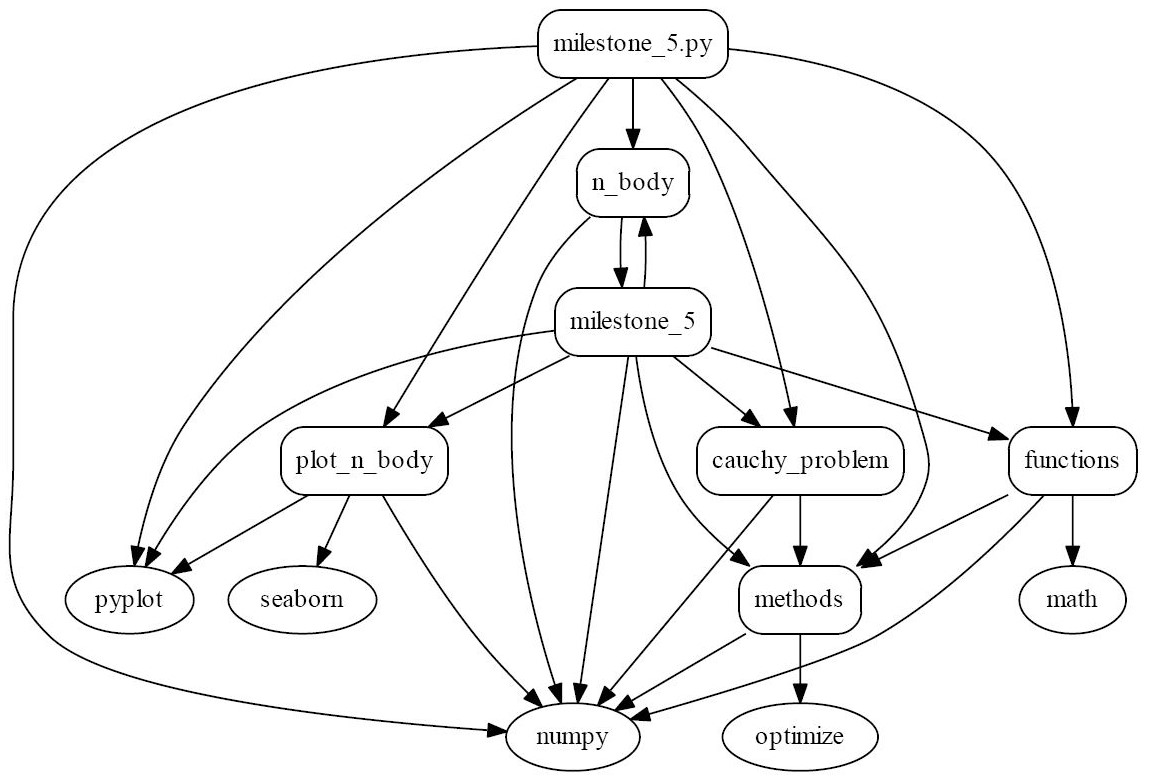
\includegraphics[width=0.90\textwidth]{FIGURES/mil5/codigo/diagram_mil5.JPG}
	\caption{Diagrama módulos Milestone 5.}
	\label{diagram_mil5}
\end{figure}

Como puede observarse en la Figura \ref{diagram_mil5} para hacer funcionar este programa se debe ejecutar el programa principal denominado $milestone\_5.py$. Este programa se encarga de llamar al resto de funciones definidas en los respectivos archivos.

Se van a comentar las nuevas funciones implementadas para la resolución de este problema.


\subsection{milestone\_5.py}
En el archivo principal se ha definido un código para iniciar las condiciones iniciales. Posteriormente se selecciona el método de resolución, para las simulaciones de ha elegido el método de Runge-Kutta de orden 4, y se ejecuta el programa de cálculo numérico. Y por último, se ejecutan las funciones que se encargan de dibujar los resultados.
\begin{figure}[H]
	\centering
	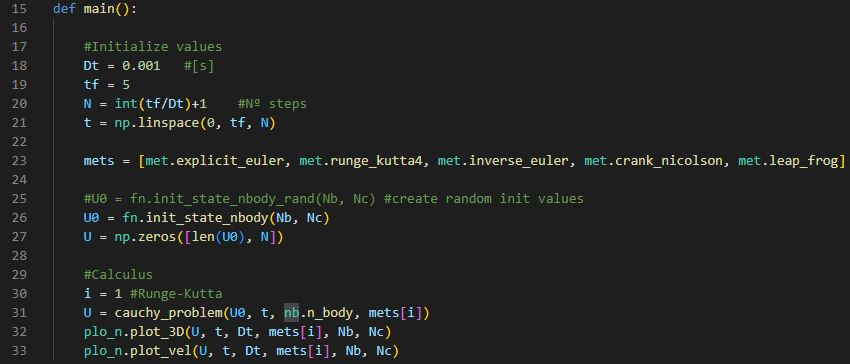
\includegraphics[width=0.95\textwidth]{FIGURES/mil5/codigo/main_1.JPG}
	\caption{Código principal Milestone 5.}
	\label{main_1}
\end{figure}


\subsection{functions.py}
En esta función se definen las condiciones iniciales de posición y velocidad de los distintos cuerpos implicados en la simulación.
\begin{figure}[H]
	\centering
	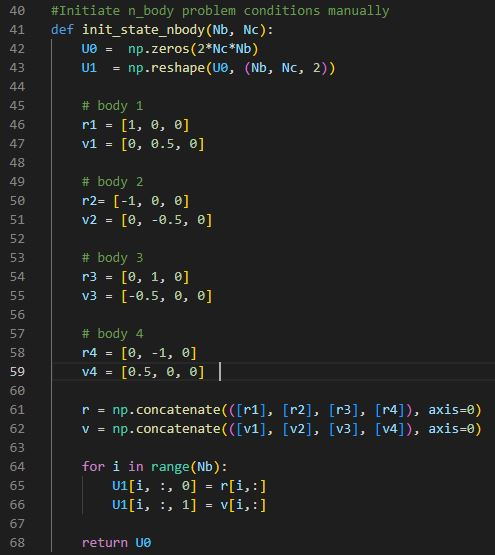
\includegraphics[width=0.7\textwidth]{FIGURES/mil5/codigo/init_1.JPG}
	\caption{Código función definir condiciones iniciales.}
	\label{init_1}
\end{figure}


\subsection{plot\_n\_body.py}
En el siguiente código se muestra la función encargada de dibujar en 3 dimensiones las trayectorias calculadas previamente.

Se ha definido un bucle que recorre todos los cuerpos del problema y dibuja en cada interacción la trayectoria asociada al cuerpo correspondiente. Destacar que se dibuja un punto que destaca sobre el resto en el punto final, para indicar la posición final del cuerpo una vez terminada la simulación. 
\begin{figure}[H]
	\centering
	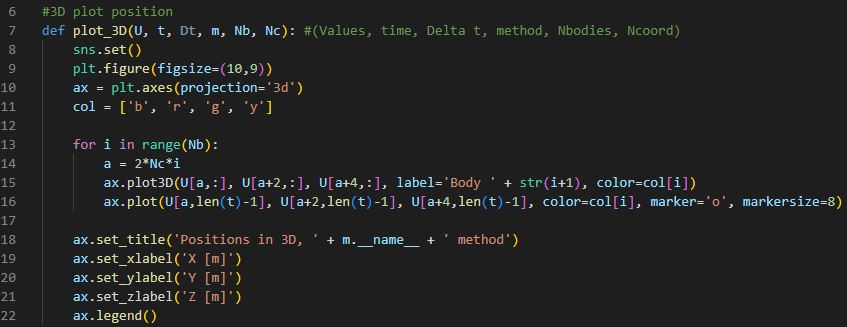
\includegraphics[width=0.9\textwidth]{FIGURES/mil5/codigo/plot_n_body_1.JPG}
	\caption{Código función dibujar trayectorias cuerpos en 3D.}
	\label{plot_n_body_1}
\end{figure}


Con el siguiente código se permite dibujar el módulo de velocidad a lo largo del tiempo de simulación. Dentro de esta misma función y por simplificar el código, se ha calculado dicho módulo a partir del vector de estados del sistema que evoluciona a través del tiempo. 
\begin{figure}[H]
	\centering
	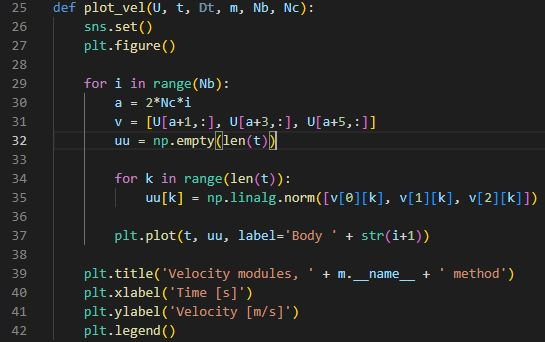
\includegraphics[width=0.9\textwidth]{FIGURES/mil5/codigo/plot_n_body_2.JPG}
	\caption{Código función dibujar módulos velocidades de los cuerpos.}
	\label{plot_n_body_2}
\end{figure}


\subsection{n\_body.py}
En el siguiente código se muestra la función que define el problema de los N cuerpos. 
\begin{figure}[H]
	\centering
	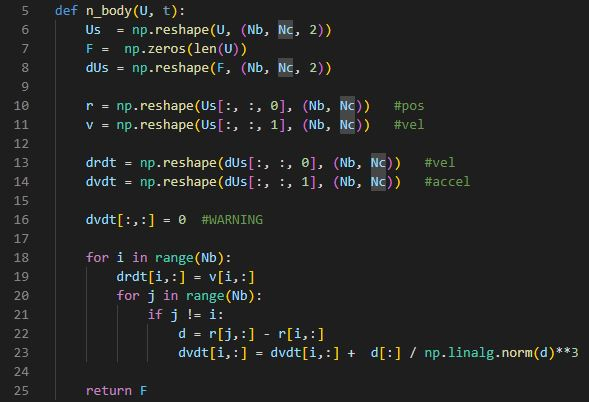
\includegraphics[width=0.75\textwidth]{FIGURES/mil5/codigo/n_body_1.JPG}
	\caption{Código función problema de los n-cuerpos.}
	\label{n_body_1}
\end{figure}



\section{Resultados y análisis}
Se han realizado un total de 3 simulaciones con distinto número de cuerpos implicados. El análisis de los resultados se muestra a continuación.

Para todas las simulaciones se ha utilizado el método de resolución numérico de Runge-Kutta de orden 4, por ser uno de los más precisos dentro de los métodos de integración que se han desarrollado en los trabajos anteriores. 

Se ha elegido un $\Delta t = 0.001$ [s] para todas las simulaciones y un tiempo de 5 segundos. Considerando que este tiempo es suficiente para obtener unos resultados decentes y visualmente aptos para analizar los resultados.

\subsection{2 cuerpos}
En la Figura \ref{2_body_3D} se pueden observar las trayectorias de los 2 cuerpos implicados en la simulación en un escenario en 3 dimensiones. 

Se han pintado los 3 ejes cartesianos y el punto que destaca sobre el resto en cada una de las trayectorias indica la posición del cuerpo en el instante final de la simulación.
\begin{figure}[H]
	\centering
	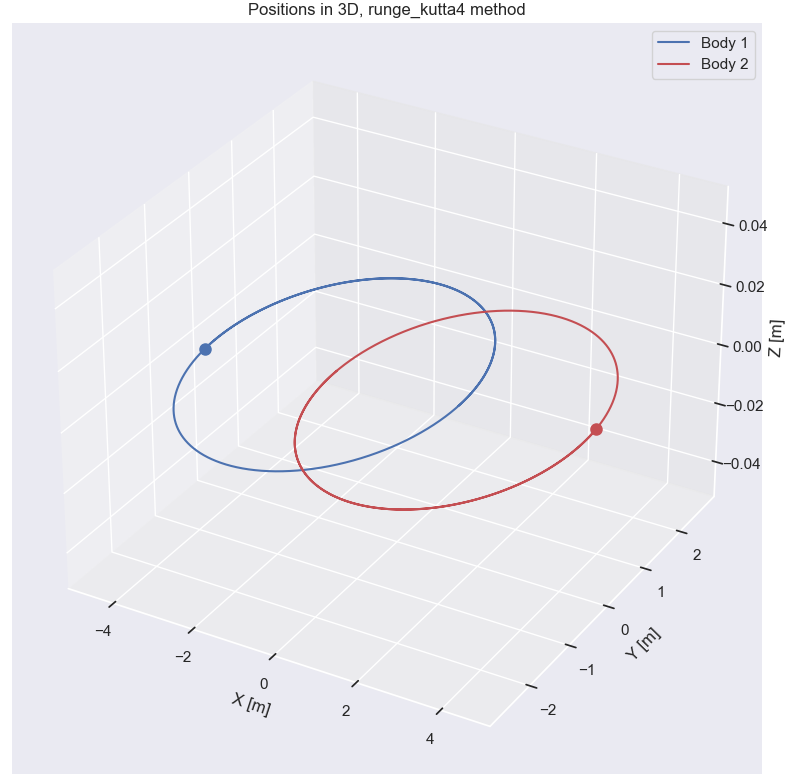
\includegraphics[width=0.90\textwidth]{FIGURES/mil5/2nb_plot3D.png}
	\caption{Trayectorias 2 cuerpos.}
	\label{2_body_3D}
\end{figure}

En la Figura \ref{2_body_vel} se muestra el módulo de velocidades de cada uno de los cuerpos partícipes a lo largo del tiempo. Para la obtención de este módulo se ha utilizado una función definida en el código de la Figura \ref{plot_n_body_2}.
\begin{figure}[H]
	\centering
	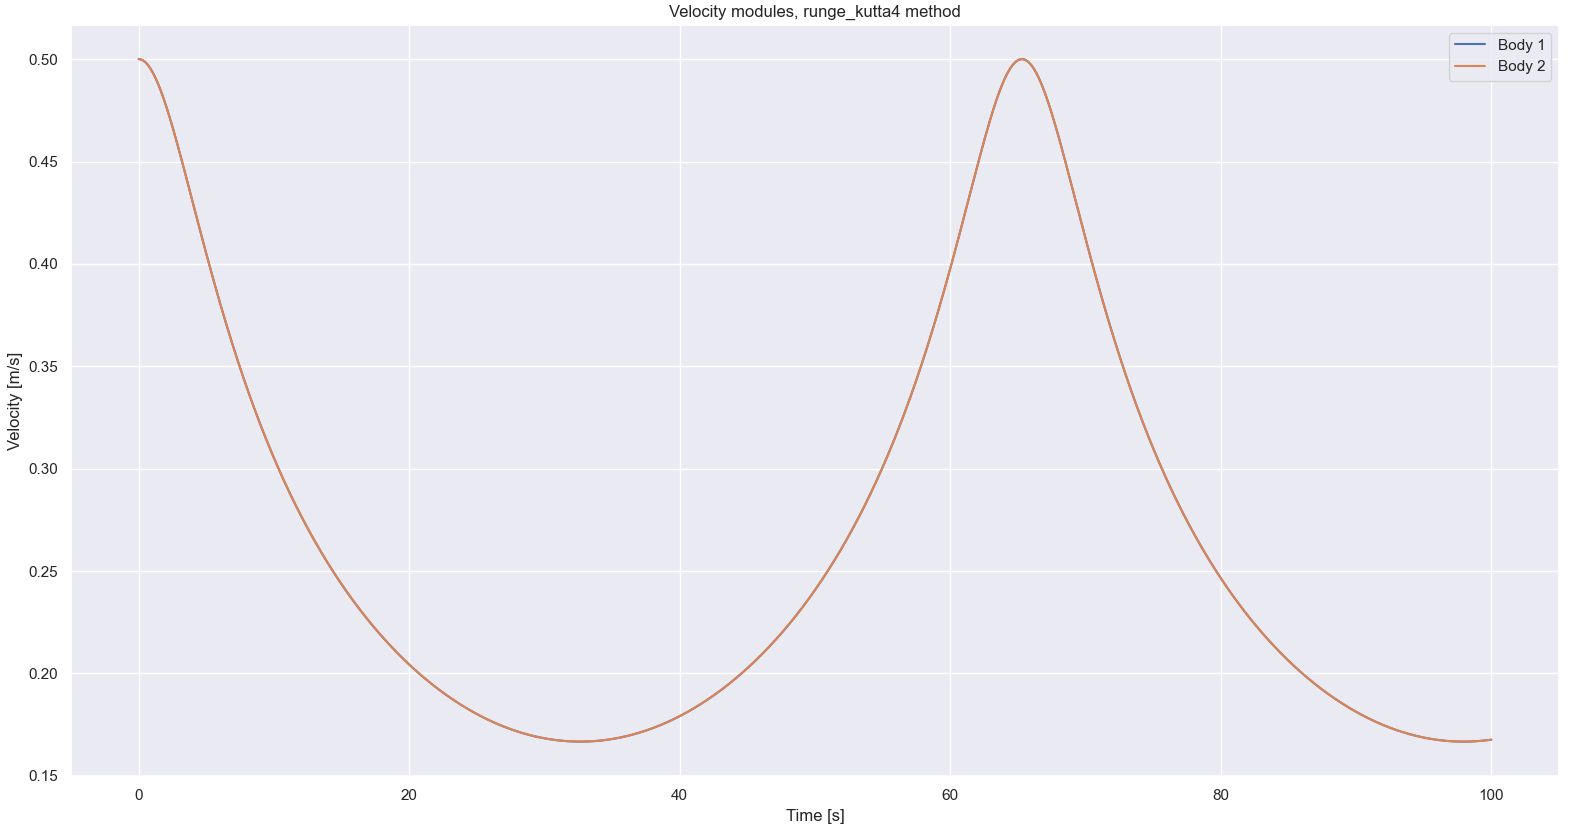
\includegraphics[width=0.90\textwidth]{FIGURES/mil5/2nb_vel.png}
	\caption{Perfil de velocidades 2 cuerpos.}
	\label{2_body_vel}
\end{figure}


\subsection{3 cuerpos}
En la Figura \ref{3_body_3D} se muestran las trayectorias que siguen los 3 cuerpos definidos para esta simulación. 

Como se puede apreciar, se observan como se afectan entre ellos los cuerpos y como modifican su trayectoria en función de la presencia de otro cuerpo cercano a él.
\begin{figure}[H]
	\centering
	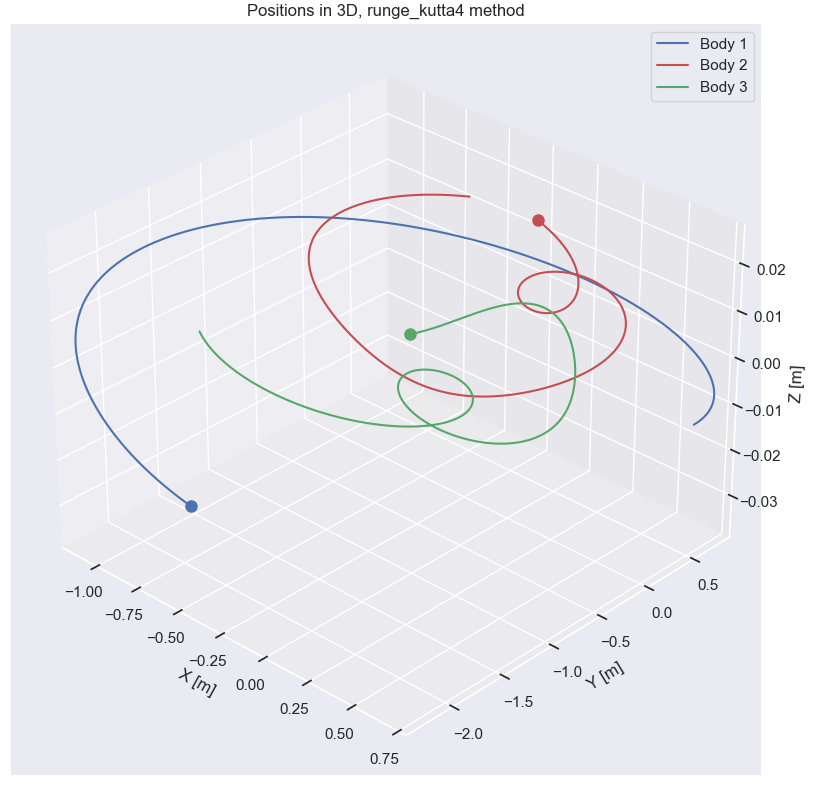
\includegraphics[width=0.90\textwidth]{FIGURES/mil5/3nb_plot3D.png}
	\caption{Trayectorias 3 cuerpos.}
	\label{3_body_3D}
\end{figure}

En la Figura \ref{3_body_vel} se observa la variación de la velocidad absoluta de cada cuerpo en función del tiempo. Se puede apreciar más en detalle como los cambios de trayectoria afectan a la velocidad de cada cuerpo y como esta se modifica.
\begin{figure}[H]
	\centering
	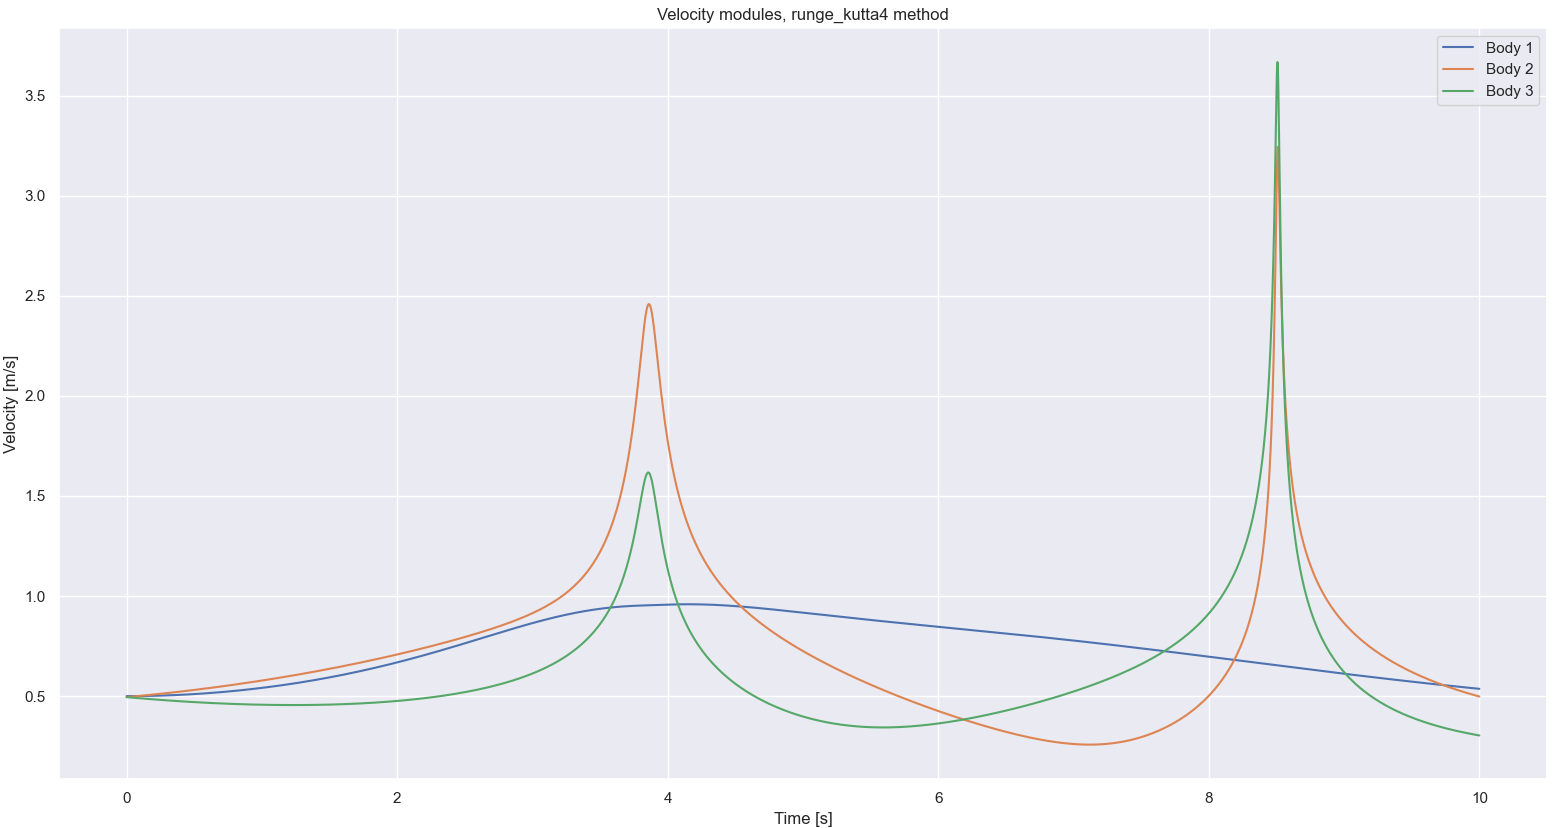
\includegraphics[width=0.90\textwidth]{FIGURES/mil5/3nb_vel.png}
	\caption{Perfil de velocidades 3 cuerpos.}
	\label{3_body_vel}
\end{figure}


\subsection{4 cuerpos}
Se han realizado dos simulaciones con 4 cuerpos implicados en la simulación con condiciones iniciales distintas de velocidad y de posición. 

En la primera simulación (Figuras \ref{4_body_3D} y \ref{4_body_vel}) con 4 cuerpos se puede observar que el movimiento de los cuerpos es mucho más aleatorio, pero aún así se puede apreciar como se afectan entre sí los cuerpos y como se provoca un cambio de trayectoria y velocidad cada vez que esto ocurre.
\begin{figure}[H]
	\centering
	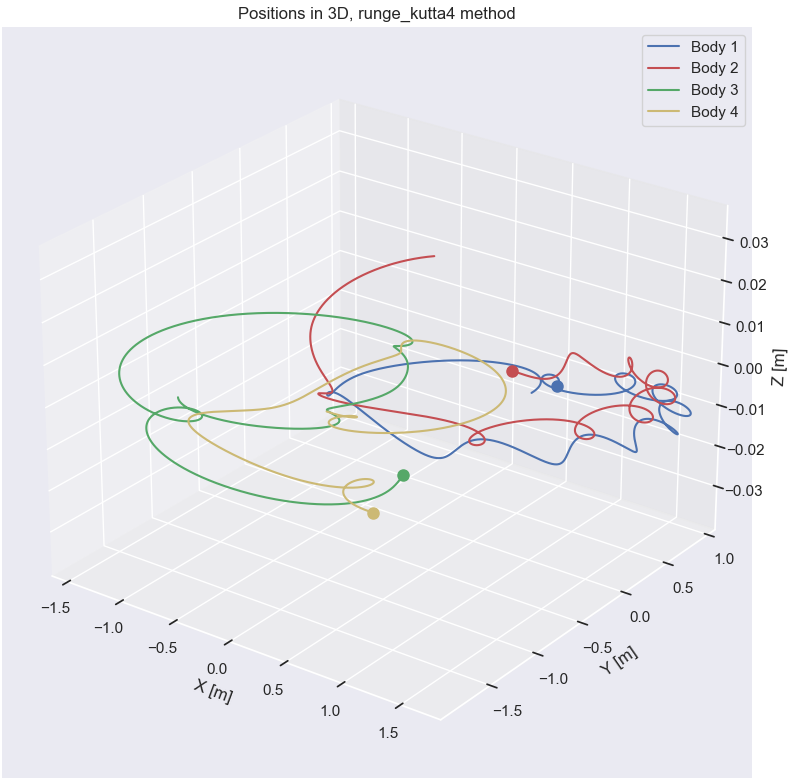
\includegraphics[width=0.90\textwidth]{FIGURES/mil5/4nb_plot3D_1.png}
	\caption{Trayectorias 4 cuerpos.}
	\label{4_body_3D}
\end{figure}
\begin{figure}[H]
	\centering
	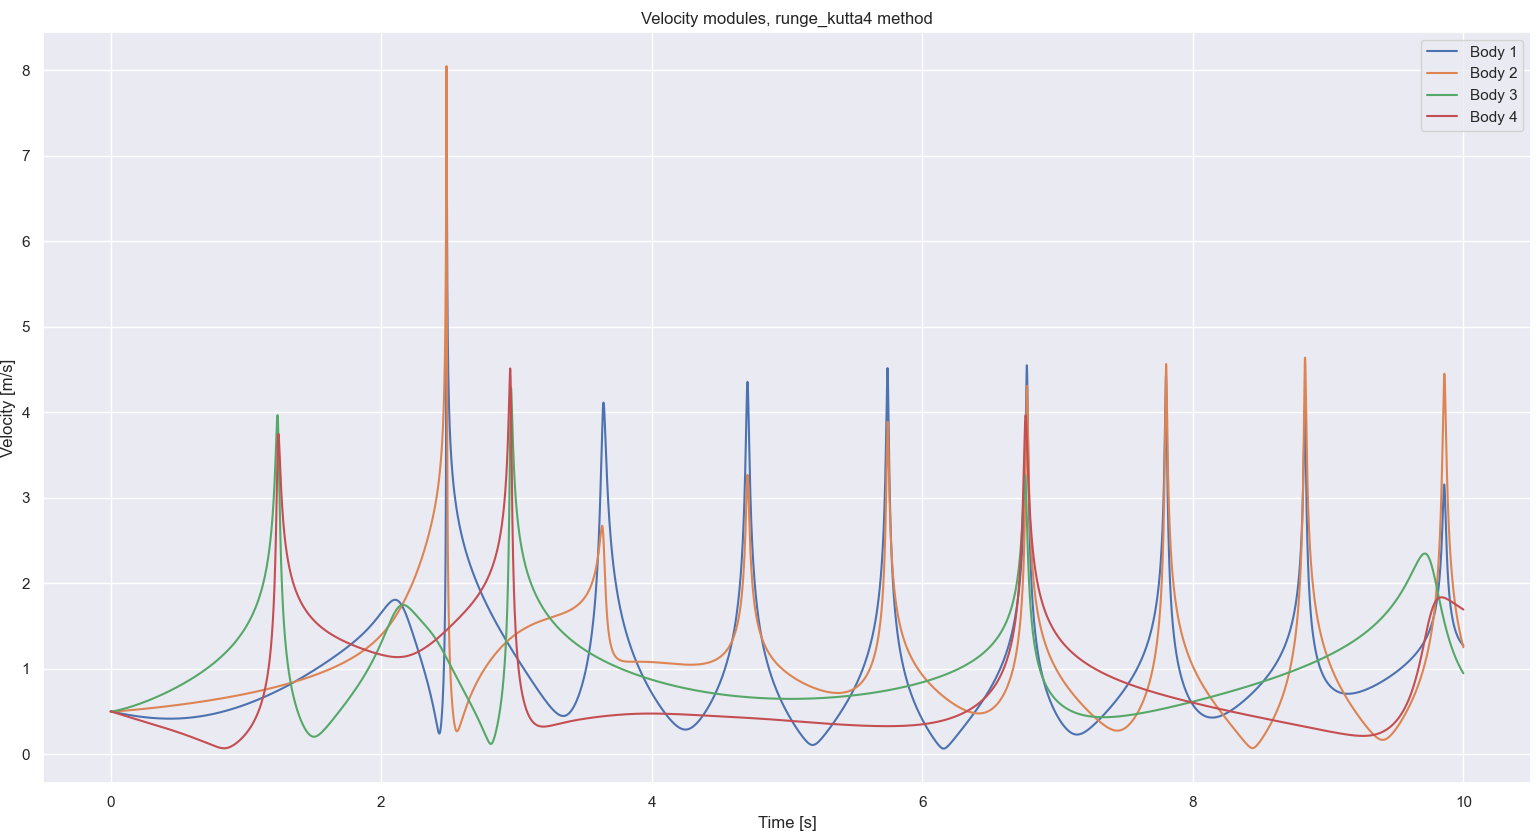
\includegraphics[width=0.90\textwidth]{FIGURES/mil5/4nb_vel_1.png}
	\caption{Perfil de velocidades 4 cuerpos.}
	\label{4_body_vel}
\end{figure}

En esta segunda simulación (Figuras \ref{4_body_3D_2} y \ref{4_body_vel_2}) se han introducido unas condiciones iniciales propensas para que a lo largo de la simulación se dibujen 4 órbitas que interactúan entre sí. El resultado se muestra en la figura siguiente, se muestra las trayectorias en 3D y la evolución de la velocidad de cada cuerpo a lo largo del tiempo de la simulación.
\begin{figure}[H]
	\centering
	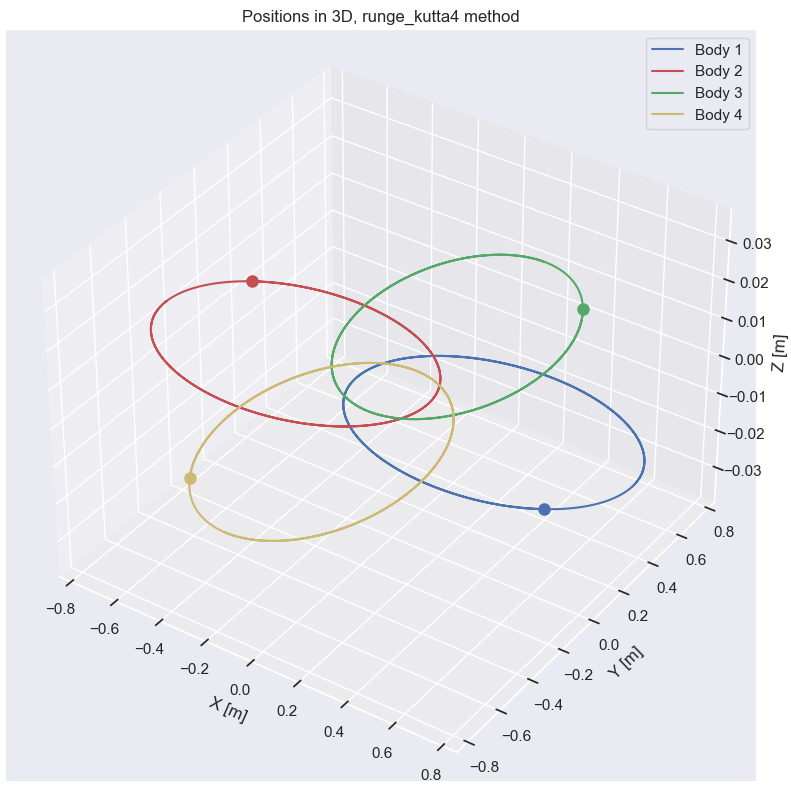
\includegraphics[width=0.90\textwidth]{FIGURES/mil5/4nb_plot3D_2.png}
	\caption{Trayectorias 4 cuerpos.}
	\label{4_body_3D_2}
\end{figure}
\begin{figure}[H]
	\centering
	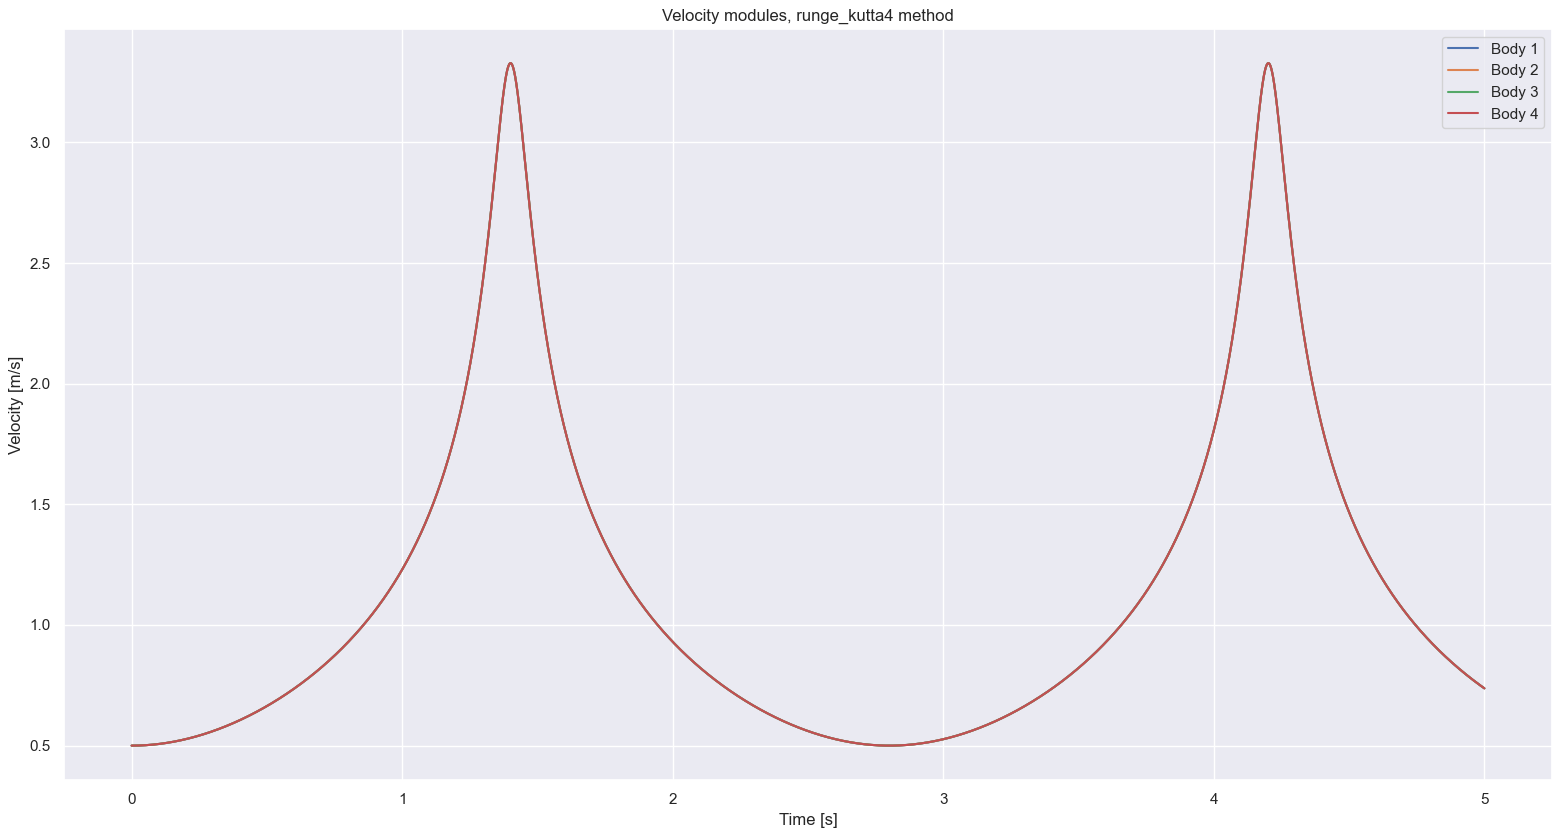
\includegraphics[width=0.90\textwidth]{FIGURES/mil5/4nb_vel_2.png}
	\caption{Perfil de velocidades 4 cuerpos.}
	\label{4_body_vel_2}
\end{figure}



\section{Conclusiones}
El iniciar los cuerpos con unas condiciones iniciales de velocidad en cada uno de los ejes ha supuesto tener que iterar con varias simulaciones hasta conseguir una simulación con unos resultados aceptables visualmente y que no convergieran todos los cuerpos al mismo punto para luego divergir. 



\end{document}
